\section{Event Reconstruction}
The event reconstruction software has been designed and developed within the CLARA framework.
As discussed in Sec.~\ref{sec:framework}, the reconstruction of events for CLAS12 is separated into micro-services that execute data processing algorithms.
%%%%%%%%%%%%%%%%%%%%%%%%%%%%%%%%%%%%%%%%%%%%%%%%%%%%%%%%%%

\begin{figure*}
\centering
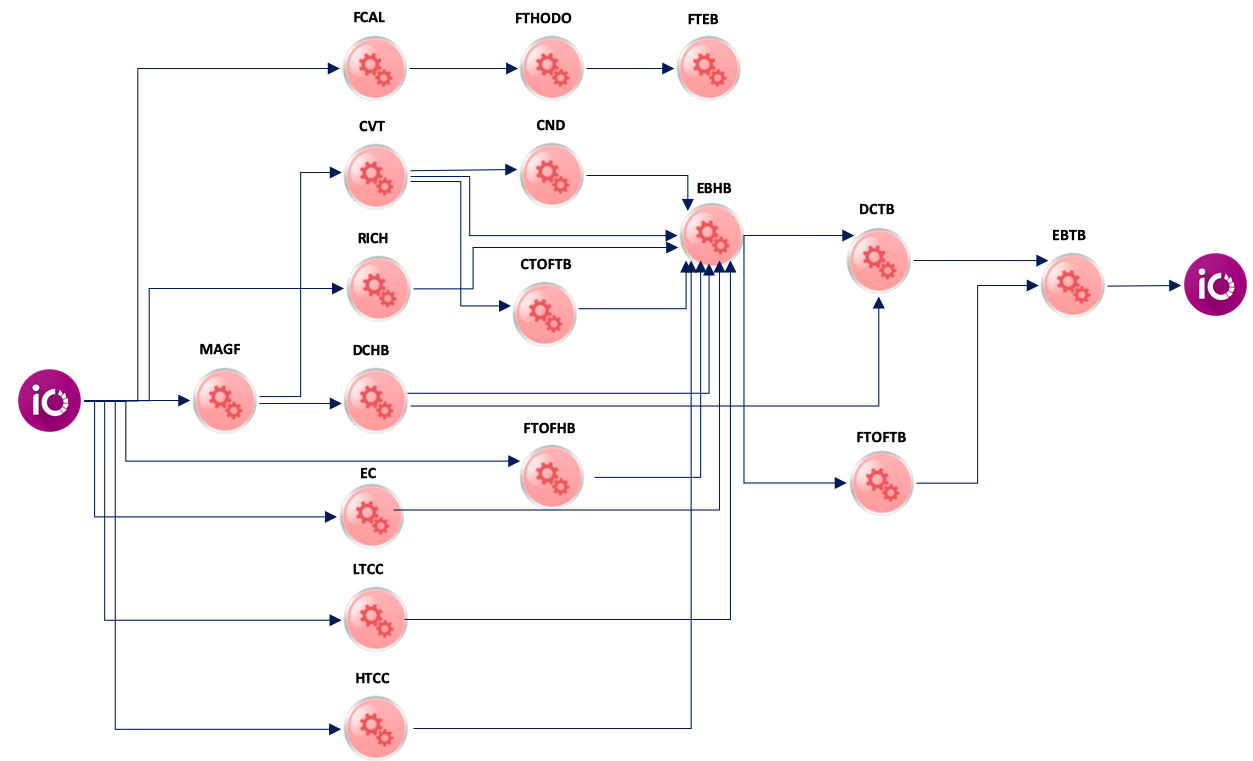
\includegraphics[width=0.7\textwidth]{pics/ServiceComposition.png}
\caption{CLAS12 reconstruction application service composition in case of sub-event level parallelization.
In this case within the event different detector component reconstruction services are processing in parallel.}
\label{fig:services}
\end{figure*}


%%%%%%%%%%%%%%%%%%%%%%%%%%%%%%%%%%%%%%%%%%%%%%%%%%%%%%%%%%%
The data reader services accesses the detector decoded data stored in a tabular structure,
called ``bank''. Each entry for decoded
detector hits is a row in a bank. A row includes detector element identifiers (sector, layer, component and order), and digitized detector data, such as signal charge, amplitude, time or pedestal, depending on the specific system. Similar bank structures are created at the decoding stage for the various information needed for event reconstruction, such as hits, clusters, tracks, etc.
The micro-services that implements reconstruction algorithms pertaining to a CLAS12 subsystems fill these banks
that are subsequently appended and written out to a file by a data-persistency micro-service.

The services running the reconstruction algorithms access the various banks (transient data) as input
and produce output banks needed for the subsequent algorithms in the reconstruction chain.
The order in which services are chained reflects the overall CLAS12 event reconstruction sequence and subsystems dependencies. First, charged particle tracks are reconstructed in both central and forward detectors based on the position of the hits detected in the relevant detectors. In parallel, hits recorded in the other detectors are processed to reconstruct the energy and time of the associate particle interaction. These are matched to the reconstructed tracks by the Event Builder service, based on geometry and time information; unmatched hits are retained as neutral particle candidates. At this stage, the Event Builder can reconstruct the event ``start time'', i.e. the time of the interaction between the beam and target particles, and identify the reconstructed particles. Once the event start time is determined, a second iteration of forward tracking can be performed to implement the so-called ``time-based-tracking''. The improved particle tracks from this step are the input for a second pass of the Event Builder, which leads to the final event reconstruction. Given this sequence, some services can run in parallel while others need the reconstruction output provided by the preceding ones.
For instance hit-based for the central (CVT service) and for forward (DCHB service) tracking
can run in parallel, while time-based tracking (DCTB) for forward tracking must come after the first execution of the event builder service.
An  overview of the reconstruction application service composition, detailing these dependencies, is shown in figures~\ref{fig:clara-overview} and~\ref{fig:services}.



